\paragraph{A current round-clock window.}
\Cref{fig:round-phase-budget} separates measured phase intervals from
the remaining recorded wall time in a later timing-only snapshot.

\begin{figure*}[!t]
  \setlength{\abovecaptionskip}{4pt}
  \centering
  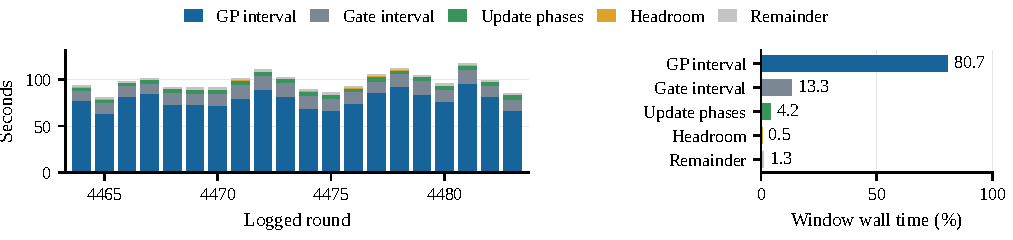
\includegraphics[width=\linewidth,height=1.60in,keepaspectratio]{figures/fig_round_phase_budget.pdf}
  \caption{\textbf{The GP interval dominates the captured round clocks.}
  All 20 completed summary records in rounds 4464--4483, captured at
  18:25 UTC on 3 November 2026. Left: recorded wall seconds by round.
  Update phases sum forward/target construction, backward/optimizer work
  and slate assembly. Remainder is the recorded wall clock minus all six
  logged phase clocks, without assigning it to a task. Right: each component's
  summed seconds divided by the \num{1944.80}\,s window total.
  The clocks include work and waits and omit gaps between rounds; they do
  not measure proposal latency, deployment throughput or learning gains.
  No quality scores enter this timing view. Scope: \cref{sec:method-status}.}
  \label{fig:round-phase-budget}
\end{figure*}
